\chapter{医疗数据处理智能体}

\section{数据输入与处理目标}

医疗数据处理智能体向用户提供数据集探查、文件上传、医疗内容处理和状态查询。
当前发布配置绑定 5 项工具，
覆盖文本上传、数据集检查、算子查询、混合处理和进度查询。
用户提交 DataMate 数据集名称或标识后，
服务解析为平台数据集标识，读取处于可处理状态的文件清单，
再按文件内容与扩展名确定处理分支。任务一的目标是登记可供知识抽取的交付数据集，并同时返回规范化文本、原有字段结构、文件级处理状态、质量记录和来源记录。

任务一接收 TXT、CSV、JSON、JSONL 和 PDF 五类输入，
其中 Markdown 按文本处理，TSV 按表格处理。
系统把文件识别、格式分组、医疗内容处理、DataMate 子数据集创建、
算子任务执行、结构恢复、质量检查和交付数据集登记组织为一条服务流程，
见图~\ref{fig:task1-pipeline}。

\begin{figure}[H]
\centering
\resizebox{0.98\textwidth}{!}{\begin{tikzpicture}[node distance=5mm and 5mm]
  \node[reportbox,minimum width=2.5cm] (source) {DataMate\\源数据集};
  \node[reportbox,right=of source,minimum width=2.7cm] (inspect) {文件探查\\格式分组};

  \node[reportbox,right=8mm of inspect,yshift=11mm,minimum width=4.1cm] (text)
    {TXT 与 PDF 文本\\清洗算子链};
  \node[reportbox,right=8mm of inspect,minimum width=4.1cm] (table)
    {CSV 表格\\保结构算子链};
  \node[reportbox,right=8mm of inspect,yshift=-11mm,minimum width=4.1cm] (object)
    {JSON 与 JSONL\\保结构算子链};

  \node[reportbox,right=8mm of table,minimum width=2.9cm] (collect) {质量检查\\结果汇聚};
  \node[reportdata,right=of collect] (result) {交付数据集};
  \node[reportbox,below=9mm of collect,minimum width=4.1cm] (status)
    {执行记录：文件状态、产物标识、质量摘要};

  \draw[reportarrow] (source.east) -- (inspect.west);
  \draw[reportarrow] (inspect.east) -- ++(4mm,0) |- (text.west);
  \draw[reportarrow] (inspect.east) -- (table.west);
  \draw[reportarrow] (inspect.east) -- ++(4mm,0) |- (object.west);

  % 三条格式分支先汇入质量检查左侧的合流点，避免与执行记录箭头重叠。
  \coordinate (qualitymerge) at ($(collect.west)+(-5mm,0)$);
  \draw[reportline] (text.east) -| (qualitymerge);
  \draw[reportline] (table.east) -- (qualitymerge);
  \draw[reportline] (object.east) -| (qualitymerge);
  \draw[reportarrow] (qualitymerge) -- (collect.west);
  \draw[reportarrow] (collect.east) -- (result.west);
  \draw[reportarrow] (collect.south) -- (status.north);
\end{tikzpicture}
}
\caption{医疗数据处理流程}
\label{fig:task1-pipeline}
\end{figure}

\section{任务探查与状态跟踪}

探查服务按 DataMate 文件记录读取文件名、类型和预览内容，
汇总五类格式的文件数，并把未支持文件保留在结果清单中。
Nexent 根据用户表达选择“查看数据集”“启动处理”或“查询运行状态”；
进入处理后，具体算子组合由服务端格式映射表决定。
同一批文件因此只产生一份任务级计划，
计划中列出每个格式分组、所用算子链、临时数据集和目标文件形式。

同步处理适用于不超过 50 个文件的数据集。
文件数更大时服务建立后台运行记录并立即返回运行标识，
状态查询依次给出排队、运行、成功或失败，
使长任务不占用一次对话请求。

任务一智能体按用户表达区分三类动作：
查看数据集时调用\path{inspect_dataset}，
执行混合格式清洗时调用\path{run_task1_mixed_cleaning}，
查询后台进度时调用\path{get_task1_mixed_cleaning_status}。
用户直接提供原始文本时，
智能体先调用\path{upload_text_to_datamate}取得真实数据集标识，
再把该标识传给数据集探查和清洗工具。

智能体只负责选择任务级工具并传递真实标识。
工具服务读取文件清单后，
由格式映射表决定文本、表格、结构化文件和 PDF 的处理链，
因此模型不会绕过结构校验直接指定算子。
工具返回\texttt{run\_id}时，
智能体继续查询状态；返回错误时，
回答保留错误阶段和已完成分组，部分产物仍按服务状态标记。

\section{文本治理与结构保持}

五类格式共享字符级基础治理，
包括表情符号、URL、乱码、不可见字符、全半角、繁简体、HTML 标记和空白规范。
文本分支继续执行长度、重复短语、特殊字符和重复文件过滤，
再进行医疗术语与缩写规范、语义噪声处理。
结构化分支只清理文本字段，并在结果汇聚阶段恢复原有结构。

医疗术语规范由 MedicalTermNormalizer 算子执行，
采用词典优先、LLM 兜底的混合策略。
词典数据来自瑞金糖尿病研究中的医学术语和通用医学缩写库，
共 114 条映射（\repoPath{operators/medical\_term\_normalizer/term\_kb.db}），
覆盖“T2DM→2型糖尿病”“AMI→急性心肌梗死”等高频缩写。
词典命中后直接替换，未覆盖的缩写交由 LLM 补充处理，
LLM 调用失败时退回词典结果。
算子返回每条替换的原文、替换后文本和出现次数。

语义噪声处理由 LLMNoiseFilter 算子执行。
该名称沿用算子注册名，当前实现读取 SQLite 规则库
（\repoPath{operators/llm\_noise\_filter/noise\_kb.db}）中通过审核并启用的规则。
规则素材来源于 cMedQA2 中文医疗问答社区数据，
覆盖广告营销、联系方式、系统导出标记、测试数据标记、网页尾部信息和 URL 链接等噪声类型。
算子将文本逐条匹配规则，命中段落按规则指定的范围（行、句子或文本块）移除，
并记录拦截类型、匹配规则和移除内容，形成文件级质量记录。
规则库独立于算子代码，新增规则只需更新数据库，
无需修改算子逻辑或重新注册。

固定规则无法提前列出病历中不断出现的闲聊和交接文字。
系统因此记录教师清洗前后的差异，并从历史差异中寻找重复片段。
同一片段至少出现 3 次、类别位于安全清单、且不含疾病、症状、药物或医学数值时，
系统才将它写入规则库。后续文件直接复用该规则，不再重复调用模型。
这项机制学习的是经过确认的重复噪声模板，不把未见表达误报为已经掌握的语义能力。

服务只报告算子实际返回的处理项，不根据提示词推测清洗效果。字符变化、解析错误、空文本、重复内容和结构复核共同组成文件级质量摘要。

服务端在 \texttt{mcp\_server/task1/chains.py} 中维护格式到算子链的映射。
文本和 PDF 复用基础清洗、文档质量检查、MedicalTermNormalizer 与 LLMNoiseFilter；
CSV 进入 TableColumnCleaner，JSON 和 JSONL 进入 JsonFieldCleaner。
PDF 先由 MinerU 转换为 TXT，再复用文本链，
因此 PDF 解析属于输入适配，医疗内容治理仍由 DataMate 算子完成。

\begin{table}[H]
\centering
\caption{医疗内容治理与结构处理方式}
\label{tab:task1-format-routing}
\begin{tabularx}{\textwidth}{L{1.7cm}L{5.2cm}Y}
\toprule
\textbf{格式} & \textbf{处理单元与算子组合} & \textbf{交付结构} \\
\midrule
TXT &
整篇或分段文本；基础治理、文档质量过滤、医疗术语与缩写规范、语义噪声处理 &
合并分段并输出 TXT \\
\addlinespace
CSV &
保留表头与行列位置；基础清理后执行表格列清理 &
保持列名、列顺序和 CSV 格式 \\
\addlinespace
JSON &
递归处理对象与数组中的文本值；基础清理后执行 JSON 字段清理 &
保持键名、嵌套层次和 JSON 对象结构 \\
\addlinespace
JSONL &
逐行解析对象并清理文本字段 &
保持一行一条 JSON 记录 \\
\addlinespace
PDF &
MinerU 提取正文并转换为文本，再执行 TXT 处理链 &
以同名 TXT 作为交付文件 \\
\bottomrule
\end{tabularx}
\end{table}

图~\ref{fig:task1-contract} 把五类输入的处理单元、格式专用步骤和交付结构展开到字段层面。
公共交付步骤负责结构恢复、重新解析检查和文件状态登记，
因此任务二能够沿同一数据集标识读取清洗结果。

\begin{figure}[H]
\centering
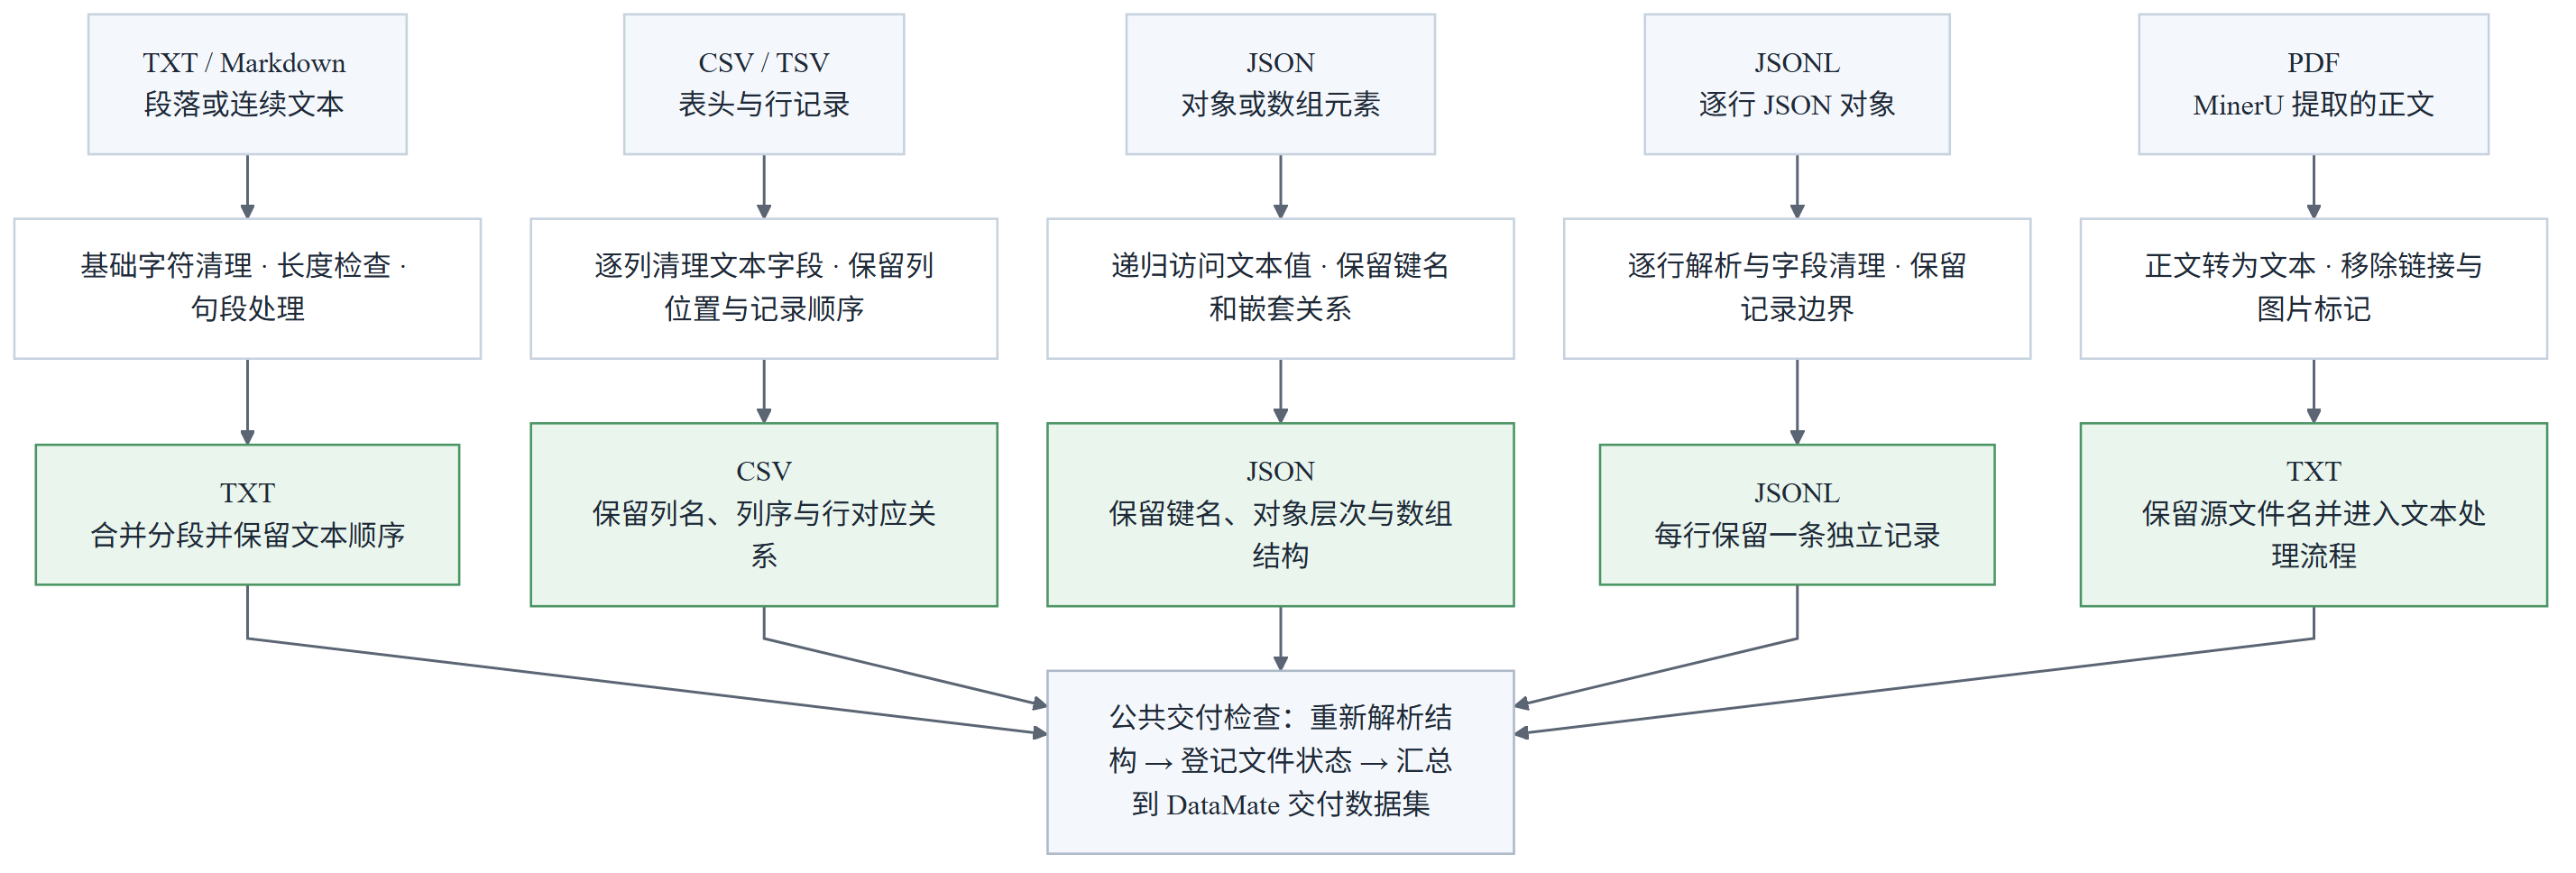
\includegraphics[width=0.98\textwidth]{figures/mermaid_format_structure.png}
\caption{五类输入的格式专用处理与结构保持结果}
\label{fig:task1-contract}
\end{figure}

文本算子可能产生带序号的分段文件，
汇聚服务按原文件名和分段序号重新合并；
JSON 与 JSONL 结果恢复扩展名后再次解析，
CSV 结果重新读取表头。
完成结构检查的文件进入最终数据集，
任务二可以继续按字段读取结构化资料。

\section{失败隔离与结果交付}

混合编排服务先按五类格式建立临时子数据集，
再为每个非空分组创建 DataMate 清洗任务。
任务返回目标数据集后，
服务读取实际产物并完成分段合并、扩展名恢复和结构检查。
各分组采用独立任务，某一格式失败时仍可保留其他分组的完成结果和文件状态。

最终交付数据集由各格式分组的合格产物重新汇聚而成。
服务将这些产物登记到一个 DataMate 数据集中，
同时返回源数据集、格式分组、算子方案、子任务、目标数据集、
文件级报告、处理性能和治理元数据。
这些字段共同说明“处理了哪些文件、经过哪条链、产物存放在哪里”，
并为任务二提供可直接解析的数据集标识。

\section{PDF 文档适配}

PDF 是任务一的文档输入适配分支，不改变后续医疗内容治理逻辑。
项目通过 MinerU 接口完成版面解析和正文提取~\cite{mineru2024,minerurepo}，
客户端负责文件上传、任务轮询和结果下载。
服务从解析产物中选择正文 Markdown，
去除版式标记后生成 TXT 文件，
再进入与普通文本相同的 DataMate 算子链。

当前适配器单次处理一份 PDF，
上传前检查文件有效性、10\,MB 大小限制和 20 页页数限制，
并为上传、轮询、结果下载、正文缺失和超时分别返回状态。
PDF 结果明确标记为文本交付，
其他格式继续保持源格式。
正文解析结果通过 Markdown 语法树提取段落与表格文字，
链接和图片标记在进入文本清洗链前被移除。

\section{交付数据与质量记录}

\begin{table}[H]
\centering
\caption{医疗数据处理智能体的交付内容}
\label{tab:task1-delivery}
\begin{tabularx}{\textwidth}{L{3.2cm}L{4.3cm}Y}
\toprule
\textbf{交付项} & \textbf{主要内容} & \textbf{后续用途} \\
\midrule
交付数据集 &
清洗后的 TXT、CSV、JSON、JSONL 文件及 PDF 转换文本 &
作为任务二知识抽取输入 \\
\addlinespace
分组任务结果 &
各格式子数据集、DataMate 任务、算子方案和目标数据集 &
查看平台任务与分支执行状态 \\
\addlinespace
文件处理记录 &
源文件、识别格式、输出文件、完成状态和处理信息 &
定位单个文件的处理结果 \\
\addlinespace
质量摘要 &
文件数、记录数、术语替换、噪声处理、格式检查和结构恢复结果 &
核对交付数据是否满足后续读取要求 \\
\bottomrule
\end{tabularx}
\end{table}

任务一把文件级算子执行组织为数据集级治理交付：
用户在 Nexent 中发起一次任务，
DataMate 承载多个格式子任务，
项目服务负责结构保持与结果汇聚，
最终得到可直接进入知识抽取的数据集入口和可核验的处理记录。
